\documentclass[runningheads]{llncs}
\usepackage{graphicx}
\usepackage{float}
\usepackage{subfigure}
\usepackage{colortbl}
\begin{document}
\title{Multisignal digital biosensors for medical applications}
\author{Maren Krafft}
\authorrunning{F. Author et al.}
\institute{Chair of technical computer science, University of Passau, Germany}
\maketitle        

      
\begin{abstract}
%es werden nicht biosensors kombiniert
Biocomputing has recently gained a place beneath other computing paradigms. Utilizing the natural rules of interaction between biochemical substances mimicking conventional computer systems, new ways and techniques of solving computing problems have been developed. This review covers the concept of biosensors, based on enzyme logic networks, that can process multiple biochemical input signals. This concept of utilizing enzymes as the ''machinery'' of biochemical logic networks, aims to create complex analytical biosensors for medical application.


\keywords{Multi-input Biosensors \and Biosensors  \and enzyme-based logic gates \and logic networks \and biomedical applications!!!!!!}
\end{abstract}


\section{Introduction}
%1.Context: what problem is being solved, why relevant or interesting, benefit, possible applications
%2.innovation: described technique completely new or does it improve earlier approcahes? what is improved 
%3.thesolution: how does the presented technique work, core idea of the solution

	In the medical field biosensors (analytic devices to convert the result of a biochemical reaction into an electric signal) are an essential tool for the monitoring and detection of a wide range of medical conditions. Biochemical substances are chemical substances that occur in natural environments like enzyme or glucose. The currently available sensors work as single-input devices, that can analyse only one specific substance. The new concept aim to create devices, that can analyse multiple inputs and transform those into a single output signal. This change allows for a variety of possible applications.\\
	
	Once realized, those biosensors are expected to revolutionize a great number of medical treatments and therapies. Through the analysis of multiple inputs, the sensors could scan specific injuries or diseases. More complex models could create sense-act-treat devices, that immediately apply the correct treatment after recognizing a specific result of the analysis. Especially in medical emergencies, where rapid reactions are of paramount importance, these developments would mark a ground-breaking change. As a further application the device could oversee the complete therapy process and analyse the impact and adjust the treatment if necessary. This repeatable mechanism is called a feedback-loop. A similar setup is already in use for Diabetes treatment. Even personalized medical therapy, which could autonomously adjust the treatment tailored to a patient’s individual needs, is imaginable.\\
	
	The basic principle of biosensors are its two layers: the receptor, that processes the biochemical input substances and the transducer, that translates the received signal into a yes/no-output. The main innovation of the new concept is the replacement of the current one-input receptor with a biocomputing network, that allows a re-creatable analysis of multiple inputs, which are then transformed into one binary output signal. The logic network, consisting of enzyme-based logic gates mimicking Boolean operations, can process biochemical information.\\
	 
	!!!!!!!As the controlled reactions provide a reliable result, this result can be transformed into a yes/no signal.
	
	This document is structures as follows. In Section 2 the concept of Biosensors with enzyme-based logic is introduced. Subsection 2.1 describes the principle of enzyme-based gates and Subsection 2.2 the networks of logic gates and the combination with transducers. While section 2 only dealy with the concept of Biosensors section 3 concentrates on the designing of multisignal Biosensors for medical applications.
	In section 4 considerations. Section 5 summarize and outlook. 
	
	
	
	
	
\section{concept}

The multisignal processing biosensors in this article are based on enzyme-based logic systems, consisting of chemical logic gates mimicking Boolean operations. Like in common biosensors with single inputs the biosensor is composed by several layers. The receptor that analyses the selected analyte of interest in common biosensors, is replaced by an enzyme logic system.
The transducer, converting biochemical interaction results into a type of signal that is oberservable, for example an electrical current. It senses physical changes and converts those into an electrical signal to represent a yes/no response.
MISSING BIOCHEMICHAL SUBSTANCES

\subsection{Enzyme-based logic gates}		
		In biocomputing, enzymes as logic gate constituents in combination with chemical inputs to create an always-the-same end product is used to mimick Boolean logic gates such as AND and OR. To digitalize chemical processes, two levels of concentrations of chemical reaction materials are considered as input signals. 0 is usually considered as the absence of a enzyme, but it can be altered. 1 equals a  significantly difference to the absence or the as 0 defined concentration.
		The result is a certain substance that acts as an output signal. If it is measurable, it signals the value 1, if not, it signals value 0.
	(Katz) \\
	
		Beispiel AND 
		In Fig 1 the enzymes glucose oxidase (short Gox. It catalyses the oxidation of glucose to hydrogen peroxide and D-glucono-δ-lactone and is often used for analysing free sugar in blood) and catalase (catalyzes the decomposition of hydrogen peroxide to water and oxygen) operate as the logic gate machinery. The two input signals are H\textsubscript{2}O\textsubscript{2} (Hydrogen peroxide) and glucose (blood sugar). When both substrates are present the inputs react and produce gluconic acid, which results in an optical absorbance change, that was defined as the ouput signal of the enzyme logic gate. The optical absorbance change just appeared in the presence of both inputs, mimicking the Boolean operation AND. 
		
		\begin{figure}[H] \centering 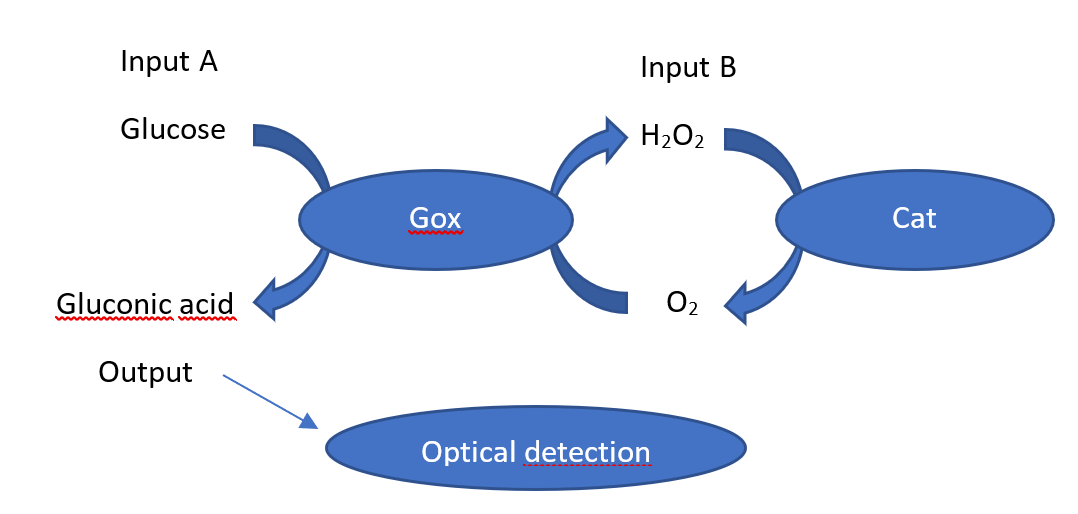
\includegraphics[scale= 0.3]{pics/ANDneu.png} \caption{Network diagramm} \label{img:and} \end{figure}
		
		\begin{center}
		\begin{tabular}{c|c|c}

			Glucose & H\textsubscript{2}O\textsubscript{2} & Output\\\hline
			0 & 0 & 0\\ 
			0 & 1 & 0\\
			1 & 0 & 0\\
			1 & 1 & 1
		\end{tabular}
		\end{center}
	
\subsection{networks with electrochemical transduction}

		By assembling these single logic gates, mimicking Boolean operations, it is possible to create small logic networks (e.g. half-adder/ half subtractor)By adding a transducer, it is possible to convert the physical change into an electric signal.
	
		Figure 1: A combination of different enzym-based logic gates, functioning as AND or OR. The cascade of reactions, when all four input chemicals are present, results in ph changes. Ph measures the degree to which a solution is acidic or alkaline. The scale is defined from 0 (acid solution) to 14 (lye solution).
		The logic network is composed of four concatenated logic gates. Those gates contain the enzymes alcohol dehydrogenase (ADH, disassembling toxic alcohols), glucose dehydrogenase( catalyst for the oxidation of glucose) and glucose oxidase act as logic gates the four specific different input signals NADH (resulting through reduction from Nicotinamid-Adenin-Dinukleotid NAD, which is a coenzyme found in all living cells),  actealdehyde (also named ethanal, which is an organic chemical compound, for example naturally occuring in coffee, bread, and ripe fruit), glucose and oxygen (O).
	 	When all inputs are present the reaction yields to an acid medium, lowering the original pH value of the solution from initial 6-7 to approximately 4.
	%erst kombination von reaktionen	
		\begin{figure}[H] \centering 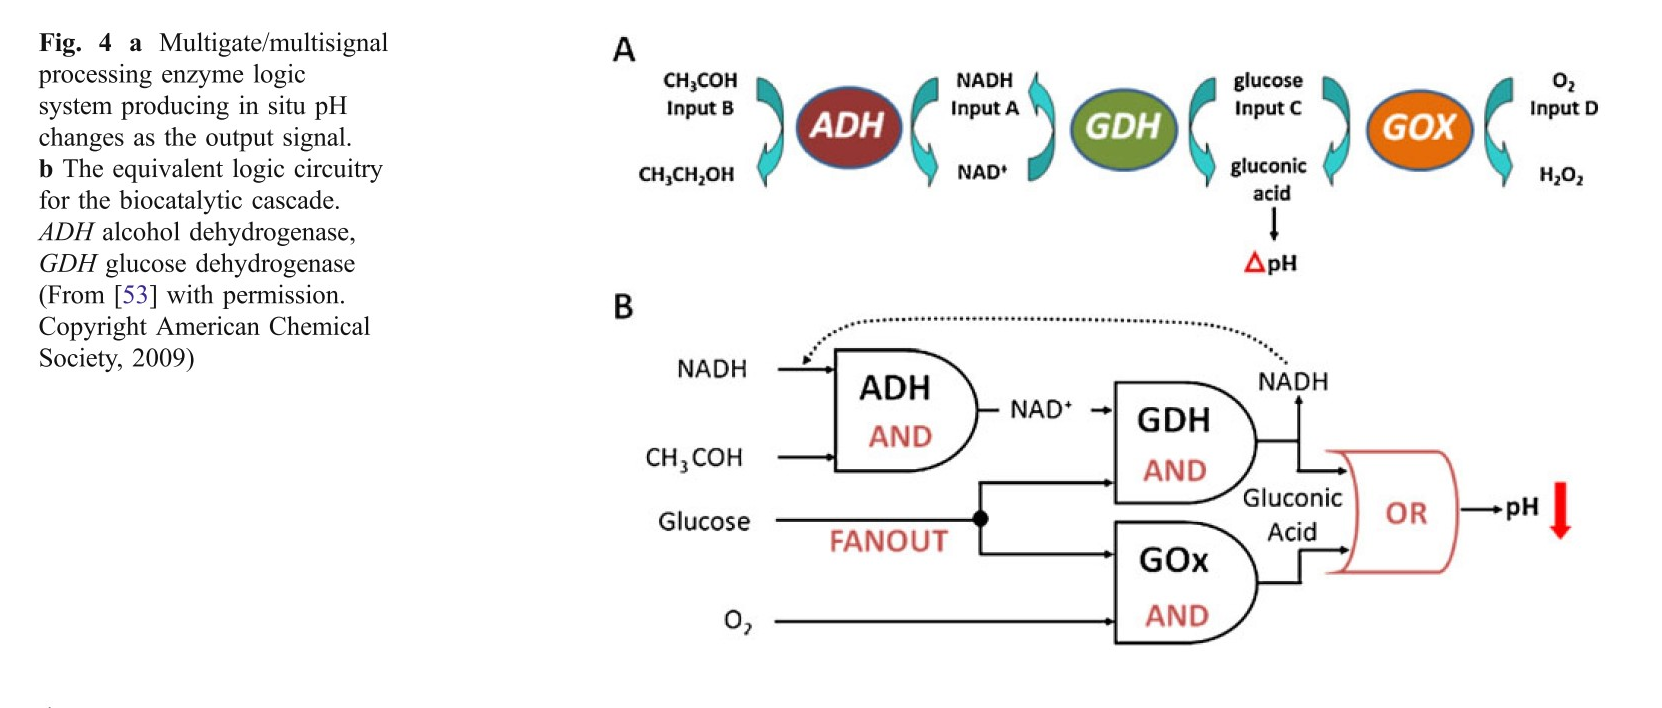
\includegraphics[scale= 0.3]{pics/biocomputing_sensor.png} \caption{Network diagramm} \label{img:grafik-test} \end{figure}
	
	%verbindung mit transducer
	
		The lower pH value resulted in switching to ON of an electrochemical interface that functioned as a transducer which makes the electrical signal readable (with low voltage as the 0-value and a defined higher voltage as 1). While 16 different combinations of input signals were possible (being present or absent) only four of those resulted in an ON state.
		\begin{figure}[H] \centering 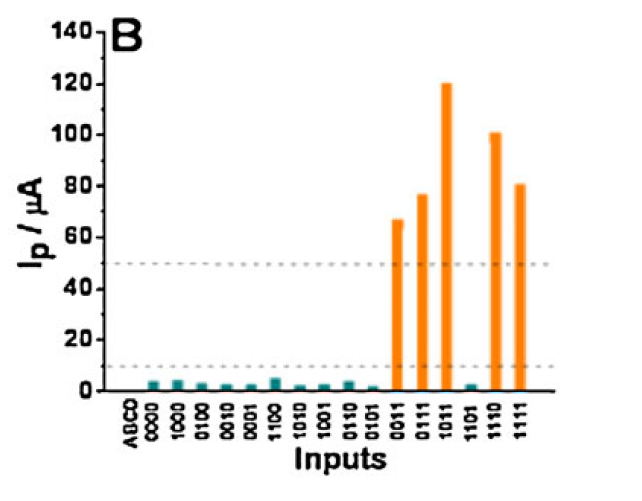
\includegraphics[scale= 0.4]{pics/ph.png} \caption{Network diagramm} \label{img:ph} \end{figure}
	
	
		This combination is an example for a multisignal processing enzyme logic system coupled with an electrochemical transduction readout of the output signal (with pH change).



\section{designing for biomedical analytic applications}
	To recognize various medical relevant conditions, it is necessary to use characteristic biochemical substances as inputs for the logic network.
	Physiological conditions resulting of a injury lead to a change in the concentration of some biochemical substances in the body, that are typical for this condition. This substances can be used as inputs for the enzyme-based network, created for the analysis.
	
	
	\subsubsection{brain injury and hemorrhagic shock}
	
	The following logical system, composed  AND and IDENTITY gates, has been designed to process information related to brain injuries and hemorrhagic shock.\
	The logic gates include the three enzymes lactate oxidase(!!!!!!), horseradish peroxidase(!!!!) and glucose dehydrogenese(!!!!!).
	As inputs it receives the three substrates glucose, lactate(!!!!) and norepinephrine()!!!!!!!! related to conditions originating from traumatic brain injury and hemorrhagic shock().\
	
	A increased glucose concentration could relate to a hemorrhagic shock, while a higher lactate concentration could either indicate a hemorrhagic shock or a brain trauma and norepinephrine can be a indicative of any traumatic injury. For the inputs 0 has been defined with the normal physiologically concentration and 1 as a abnormally increased concentration.
	
	Optical and electrochemical means were used as transducer 


	
	Especially the following combinations of input signals appeared to correspond the the two different conditions
	
	\begin{center}
		\begin{tabular}{c|>{\columncolor[gray]{0.8}}c|>{\columncolor[gray]{0.8}}c|c|c|c|}
			condition & norepinquinone & NADH & glucose & lactate & norepinephrine\\ \hline
			traumatic brain injury & 1&0&0&1&1\\
			hemorrhagic shock & 1&1 &1&1&1\\
		\end{tabular}
	\end{center}

	
	binary output
	
	
	



\section{considerations} 
Being only a concept yet, there are plenty of challenges, that must be solved until a successful realization of complex applicable biosensors. The most current are as follows.
\subsubsection{Surface confinement}	In recent research, the success of enzymatic reactions was growingly dependant on the immobilization of the reagent layer. Early experiments with enzyme logic dissolved the gate constituents and chosen inputs in a solution. With the aim of complex networks that require multiple different gate constituents and inputs, each section needs to be differentiated and isolated, to prevent cross-reactions. To achieve multiple and “stackable” logic gates, the biocomputing layer needs to be immobilized. Agglomerations of multiple logic systems also induce further challenges. All reacting components need to be carefully evaluated to prevent cross-reactions, while the outside coating of the device must simultaneously protect the reagents within the device but be permeable to the desired inputs. The impact of an immobilization on the performance of biosensing devices has yet to be examined.\\

\subsubsection{Optimal transduction}	More complex setups require better and more versatile transducers. With the universal goal of processing an arbitrary number of inputs into only one output signal, the development of versatile transducers becomes crucial. WHAT The transducer must be able to process multiple logic-gate results and yet translate those into one (optical or electrical) output signal. Current research had to apply variant transducing strategies for complex devices, but aims to develop a multipurpose transducer, which can be generally utilized.\\

\subsubsection{Defining the Boolean 0- and 1-values} In the biochemical logic system as well as for the transductiors, there has to be a defined 0 and a respectively defined 1 value. 0 should mark the biological standard value, while the state of the art is to define it as the absence of signals(!!!!!), 1 the critical value. The definition of the 1-value is also problematic. In research, the 1 value has mostly been defined as a random convenient value, instead of using applicable medically critical values. Within the same field, the difference between a relevant 0 and a relevant 1 can be minimal. This leads to difficulties with the transduction. An offered solution would be a sigmoidal signal translation rather than the usual linear, to emphasise the difference an allow more reliable reading.
Scalability		One central aim of research is to achieve a maximal flexibility of sensors. In the end, it is highly expected to be able to scale every parameter of the sensor, from the complexity of the logic system to the specificity of the transducer. The aim is, to potentially combine any given number of logic gates into networks, that create more and more complex logic systems and respectively allow new applications.

\subsubsection{Relevant inputs}	A majority of laboratory projects worked with biomedical irrelevant substances for their proof of concept. A crucial step is to make the concept work with relevant inputs. In recent studies, scientists realized networks with biomedically relevant substances as inputs. The used logic networks yet did not depict a senseful logic context to the substances(WHAT). Thus not only the work with relevant substances needs to be developed further, but also the logic networks need to be adjusted to depict relevant ???\\

\subsubsection{Challenges of drug delivery}	One slightly more distant concern is the functionality of drug delivery devices. One of the key goals of research is to develop autonomous devices, that analyse certain physiological parameters and offer an immediate reaction. Experiments have shown a need for different methods and technology to distribute the correct treatment within the cycle of those devices.


\section{Conclusion}

\begin{itemize}
	\item design of biosensoric systems with logically processes signals represented by varous biomarkers characteristic for different abnormal physiological conditions
	\item analysis of the chemical output signals generated by biomolecular logic systems is often limited.
	\item Enzyme logic system: multiassemblies to perform simple arithmetic functions
	\item idea: applicatoin of biomolecular logic system for analytical purpose new class of biosensors that accept many input signals and produce binary outputs in form yes/no 
	\item example analyse protein libraties associated with muliple sclerosis(58)
\end{itemize}

\begin{itemize}
	\item not just chronic but also ..........
	\item state of the art
	\item feedback loop currently devoted to management of diabetes through integration of an electrochemical glucose sensing element with an insulin-delivery feedback loop for the optimal dose of insulin (69-71)
	\item example analyse protein libraties associated with muliple sclerosis(58)
	
	ENzyme logic system recognizing various injury-related physiological conditions
	\begin{itemize}
		\item types of injuries result in concentrations of chemical substances in the body
		
		\item example: lactate axidase, horeserasish peroxidase and glucose dehydrogenase = designed to process biochemical information related to pathophysiological conditions from brain injury
		\item markers: glucose(hemorrhagic shock),lactate(rhagic shock or traumic brain injury) and norepinephrine(traumatic injury)
		\item logic 0 = normal concentrations
		\item change results into different numbers 1,2,3 - convenient
		\item = biocomputing logic system 
		\item challenge: difference between normal and unnormal minimal => not linear, should be sigmoidal	
	\end{itemize}
\end{itemize}
	\begin{itemize}
	\item optimal surface confinement of the biocomputing layer
	\item engineering enzyme microenvironment (transducer layer)
	\item contact between biocomputing layer and transducing surface
	\item combine individual logic-gates and maintain high enzymatic stability and reataining individual reagents
	\item leakage of cosubstrate 
	\item no cross-reactions
	\item surface confinement? layer-by layer? more efficient and rational 
	\item level of the surface confined reagents tailored for account of different input concentrations /enzyme activities 
	\item coating: optimized for transport and excluding potential interfernece and protecting the surface
\end{itemize}

\subsection{optimal transduction of biocomputing signal processes}
\begin{itemize}
	\item simultaneous measurements of multiple outputs require different transduction strategies (common: fixed potential )
\end{itemize}
\begin{itemize}
	\item Requires:interface of biocomputing systems + electronic transducer\\
	Therefore
	\item scalability (increasing nuber of logic gates, assembling into complex networks)
	\item complexity(coupling of gates abd non boolean elements)
	\item composition, preparation and immobilization of the biocomputing surface layer
	\item layer by layer
	\item optimal surface confinement 
	\item careful engineering of the enzyme microenvironment(on transducer surface) for performance
	\item biocomputing layer + transducing layer + combine individual logic-gate elements	
\end{itemize}

	good but needs lot of work\\
	sums up bla
	
		Profound impact\\
	
	Through processing automatically several biochemical inputs(physiological information), it can provide a rapid and reliable assessment of overall physiological conditions. This can help a optimal timley therapeutic intervention. They will realize sense/delivery feedback loops by coupling signal processing with chemical actuators to revolutionize patient monitoring and drug delivery. 
	
	In the Biosensors processing multiple biochemical signal, the core idea is to add a biocomputing layer that produces a final output in form of a yes/no response. Kapitel 1.2\\
	
	Chances:
	
	
	
	
	In contrast to recent biosensors, those with a 11111111111 logic promise a higher fidelity, a greater range of processable inputs, more complex applications such as sense-act-treat loops and rapid assessment of the respective substances.(mehr ausformulieren)
	
	
	
	
	\subsection{Biosensors  logic systems}
	Biosensors logically processing multiple biochemical signals\\
	-such procassed information produces a final output yes/no \\
	- boolean logic networks composed of biomolecular systems\\	
	\begin{itemize}
		\item multiple target analytes(inputs) for enzyme gates
		\item high-fidelity compared
		\item closed loop/feedback loops possible (sense/act/treat)
		\item rapid and reliable assessment of overall physiological condition
		\item could initiate optimal timely therapeutic intervention
		\item biosensors + enzyme logic gates
		\item allows direct coupling of signal processing with chemical actuators 
		\item application og biomolecular logic systems for analystic purposes could yield a novel class of biosensors: many input signals and binary outputs
		\item logically processed feedback between drug appl. and physiological conditions can signifacntly imprive drug targeting and efficiency 
		
		\item difficulties: complexity by assembling individual logic gates into complex logic networks (intelligent by molecular logic) (43-34-67)
		\item new approach for the sensor design and operation, interfach biocomputing system and electronic transducers
	\end{itemize}


\begin{thebibliography}{8}
	\bibitem{application}
	Parikha Mehrotra, Biosensors and their applications - A Review (2016) https://www.ncbi.nlm.nih.gov/pmc/articles/PMC4862100/
	
	\bibitem{biosensors}
	Daniel R. Thevenot, Klara Toth, Richard A. Durst, George S. Wilson, Electrochemical biosensors: recommended definitions and classifications In: Biosensors and Bioelectronics 16 (2001) 121- 131 https://www.sciencedirect.com/science/article/pii/S0956566301001154
	
	\bibitem{source1}
	Joseph Wang, Evgeny Katz, Digital biosensors with build-in logic for biomedical applications- biosensors based on a biocomputing concept, in: Anal Bioanal Chem(2010) 1591-1603
	
	\bibitem{source2}
	Shengbo Sang, Wendong Zhang and Yuan Zhao, State of the Art in Biosensors, in: State of the Art of Biosensors(2013) 89-110 https://www.intechopen.com/books/state-of-the-art-in-biosensors-general-aspects/review-on-the-design-art-of-biosensors
	
	\bibitem{source3}
	Evgeny Katz, Enzyme-Based Logic Gates and Networks with Outout Signals Analyzed by Various Methods, In: ChemPhysChem 16(2017), 18 1688-1713 https://onlinelibrary.wiley.com/doi/full/10.1002/cphc.201601402
	
	\bibitem{chemie}
	DónalLeechMariePellissierFrédéricBarrière, INElectrochemical Sensors, Biosensors and their Biomedical Applications (2008), Pages 385-410 https://doi.org/10.1016/B978-012373738-0.50014-3
	
\end{thebibliography}
\end{document}
